\documentclass[10pt]{beamer}

% Copia local de preamble.tex:
\usetheme[progressbar=frametitle]{metropolis}
\usepackage{appendixnumberbeamer}
\usepackage{fancyvrb}
\usepackage{booktabs}
\usepackage[scale=2]{ccicons}
\usepackage{pgfplots}
\usepgfplotslibrary{dateplot}
\usepackage{type1cm}
\usepackage{lettrine}
\usepackage{ragged2e}
\usepackage{xspace}
\newcommand{\themename}{\textbf{\textsc{metropolis}}\xspace}
\usepackage{graphicx} % Allows including images
\usepackage{booktabs} % Allows the use of \toprule, \midrule and \bottomrule in tables
\usepackage[utf8]{inputenc} %solucion del problema de los acentos.
\usepackage{xcolor}
\definecolor{LightGray}{gray}{0.9}

\usepackage{minted}
\usemintedstyle{tango}
\newcommand{\mypyfile}[1]{\inputminted[linenos=true, fontsize=\footnotesize, frame=lines, framesep=5\fboxrule,framerule=1pt]{python}{#1}}

\setminted[python]{breaklines,frame=lines,framesep=2mm,baselinestretch=1.2,bgcolor=LightGray,linenos, fontsize=\footnotesize} % obeytabs=true, tabsize=2, showtabs=true}

%%%%%%%%%%%%%%%%%%%%%%%%%%%%%%%%%%%%%%%%%%%%%%%%%%%%%%%%%%%%%%%%%%%%%%%%%%%%%%%%%%%%%%
\setbeamercolor{progress bar}{fg=blue!50!black,bg=white!50!black}
\setbeamercolor{title separator}{fg=red!50!black,bg=white!50!black}
\setbeamercolor{frametitle}{fg=white!80!black,bg=red!50!black}
\title[PCFI161]{Programaci\'on para F\'isica y Astronom\'ia}
\subtitle{Departamento de Física.}

\newcommand{\myfront}{
\author[PCFI161]{Corodinadora: C Loyola \\ Profesoras/es C Loyola / C Femenías / Y Navarrete / C Ruiz}
\institute[UNAB]{Universidad Andrés Bello}
\date{Primer Semestre 2025}
}

\titlegraphic{%
  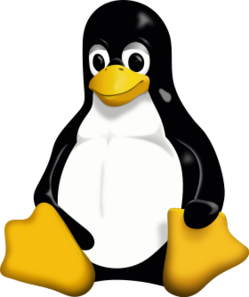
\includegraphics[width=.08\textwidth]{logo-tux.png}\hfill
  
\includegraphics[width=.3\textwidth]{logo-unab.png}\hfill
  
\includegraphics[width=.08\textwidth]{logo-python.png}
}

\makeatletter
\setbeamertemplate{title page}{
  \begin{minipage}[b][\paperheight]{\textwidth}
    \vfill%
    \ifx\inserttitle\@empty\else\usebeamertemplate*{title}\fi
    \ifx\insertsubtitle\@empty\else\usebeamertemplate*{subtitle}\fi
    \usebeamertemplate*{title separator}
    \ifx\beamer@shortauthor\@empty\else\usebeamertemplate*{author}\fi
    \ifx\insertdate\@empty\else\usebeamertemplate*{date}\fi
    \ifx\insertinstitute\@empty\else\usebeamertemplate*{institute}\fi
    \vfill
    \ifx\inserttitlegraphic\@empty\else\inserttitlegraphic\fi
    \vspace*{1cm}
  \end{minipage}
}
\makeatother


\makeatletter
\setlength{\metropolis@titleseparator@linewidth}{2pt}
\setlength{\metropolis@progressonsectionpage@linewidth}{2pt}
\setlength{\metropolis@progressinheadfoot@linewidth}{2pt}
\makeatother


\begin{document}

\myfront{}

\begin{frame}
  \titlepage
\end{frame}

\begin{frame}
  \frametitle{Resumen - Parte 1 (Semana 03)}
  \tableofcontents
\end{frame}

%----------------------------------------------------------------------------------------
%	PRESENTATION SLIDES
%----------------------------------------------------------------------------------------
\metroset{block=fill}

%------------------------------------------------
\section{Funciones, Paquetes y Módulos}

\subsection{Paquetes}

\begin{frame}{Paquetes}
Existen muchas operaciones más avanzadas que la aritmética simple:
\begin{enumerate}
	\item Multiplicar matrices.
	\item Calcular logaritmos.
	\item Hacer gráficos, etc.
\end{enumerate}

Python posee una gran variedad de \textbf{funciones} que se organizan en \textbf{paquetes}, cada uno con un nombre identificativo.

\begin{block}{Paquetes}
Colección de funciones útiles y relacionadas entre sí.
\end{block}
\end{frame}

\begin{frame}{Paquetes}
Antes de usar una función de un paquete, debemos “importarla”.
\begin{example}[\texttt{log} del paquete \texttt{math}]
\texttt{from math import log}\\
\texttt{x = log(2.5)}
\end{example}

\footnotesize
\begin{block}{algunas funciones del paquete \texttt{math}}
\begin{tabular}{ll}
\texttt{log}              & logaritmo natural (base \(e\)) \\
\texttt{log10}            & logaritmo base 10              \\
\texttt{exp}              & exponencial                    \\
\texttt{sin, cos, tan}    & seno, coseno, tangente (rad)   \\
\texttt{asin, acos, atan} & arcseno, arccos, arctan        \\
\texttt{sinh, cosh, tanh} & seno, coseno, tang. hiperbólico\\
\texttt{sqrt}             & raíz cuadrada
\end{tabular}
\end{block}
\end{frame}

\begin{frame}[fragile]{Paquetes}
Podemos examinar qué funciones incluye un paquete con \texttt{dir(paquete)}:
\begin{example}\footnotesize
\verb|>>> import math|\\
\verb|>>> dir(math)|\\
\texttt{['\_\_doc\_\_', '\_\_file\_\_', '\_\_loader\_\_', '\_\_name\_\_', '\_\_package\_\_', 
'\_\_spec\_\_', 'acos', 'acosh', 'asin', ... , 'pi', 'pow', ... 'sin', 'sqrt', 'tan', ...]}
\end{example}

\end{frame}

\begin{frame}[fragile]{Paquete \texttt{math}}
\begin{itemize}
	\item Contiene funciones menos comunes (\texttt{erf, gamma}), y también constantes como \texttt{pi} o \texttt{e}.
	\item Puedes importar varias funciones a la vez:
\begin{example}
\texttt{from math import log, exp}
\end{example}
	\item También es posible importar \textit{todas} las funciones: \texttt{from math import *}, pero esto puede generar conflictos de nombres si no se tiene cuidado.
\end{itemize}
\end{frame}

\subsection{Módulos}
\begin{frame}[fragile]{Módulos}
Algunos paquetes se dividen en submódulos. Por ejemplo, \texttt{numpy} se organiza en varios módulos:
\begin{example}[importando del módulo \texttt{linalg} de \texttt{numpy}]
\texttt{from numpy.linalg import inv}
\end{example}
Aquí \texttt{numpy} es el paquete, y \texttt{linalg} es un módulo específico.  
\end{frame}

\begin{frame}[fragile]{Poniendo en práctica: Coordenadas polares a cartesianas}
\begin{itemize}
    \item Queremos convertir \((r,\theta)\) a \((x,y)\).
    \item Fórmulas: \(x = r \cos(\theta)\), \(y = r \sin(\theta)\).
    \item Supongamos que \(\theta\) se ingresa en grados.
\end{itemize}
\begin{minted}{python}
from math import sin, cos, pi

r = float(input("Ingrese r: "))
d = float(input("Ingrese theta en grados: "))
theta = d*pi/180

x = r*cos(theta)
y = r*sin(theta)

print(f"x = {x}, y = {y}")
\end{minted}
\end{frame}

%------------------------------------------------
\section{Funciones}
\begin{frame}[fragile]{Funciones integradas y comentarios}
\begin{enumerate}
	\item \textbf{Funciones integradas}:  
	Hay un grupo de funciones que vienen “de fábrica” en Python, p. ej. \texttt{float}, \texttt{int}, \texttt{complex}, \texttt{abs}, \texttt{print}, \texttt{input}, etc.
	\item \textbf{Comentarios}:  
	Uso del símbolo “\#” para anotar explicaciones que el intérprete ignora por completo.
	\begin{example}
\# Esto es un comentario que no se ejecuta
	\end{example}
\end{enumerate}
\end{frame}

\begin{frame}
\Huge{\centerline{Fin de la Parte 1}}
\end{frame}

\end{document}

